\chapter{準備}
本章では,提案アプローチで用いるNMF,バギング,スペクトラルクラスタリングについて説明する.
\section{非負行列因子分解}
非負行列因子分解(nonnegative matrix factorization; NMF)\cite{Lee1999}は行列分解の手法の一つである.
NMFは非負行列$X \in \mathbb{R}_+^{I \times J}$を2つの非負行列の積として分解する:
\begin{equation}
	X \approx DC, \ 1 \geq K \geq \min\{I, J\}.
\end{equation}
ただし,$D \in \mathbb{R}_+^{I \times K}$,$C \in \mathbb{R}_+^{K \times J}$,$K < rank(X)$である.
このモデルを\Figref{fig:nmf-prepare}に示す.
基底数$K$は事前に決めなければいけないパラメータである.

\begin{figure}[htbp]
	\centering
	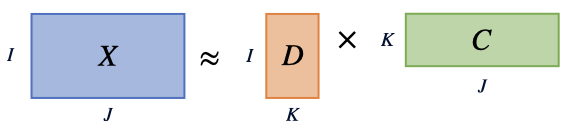
\includegraphics[width=0.8\hsize]{nmf-prepare}
	\caption{NMFのモデル.}
	\label{fig:nmf-prepare}
\end{figure}

NMFでは目的関数を最小化することによって$D$と$C$を求める.
目的関数はデータに対して置く仮定によって変わる.

\subsection{NMFの基底数}
NMFの基底数を決めるのは難しい問題である.
NMFの基底数の決め方にはいくつかのアプローチがある.
まずは,専門家や解析者の知識に基づいて決めることである.
この方法はデータに対して十分な知識がない時には使えない.

次にBIC~\cite{wasserman2000a}やAIC~\cite{Akaike1974}を用いる方法である.
これらは漸近理論に基づいた近似を行った情報量基準である.
NMFはデータが増えるほどパラメータ数$(I + J) * K$が増えるという特徴があり,これらを用いるのは本来不適切である.

次にRのNMFパッケージにも組み込まれているBrunetら~\cite{Brunet2004}の方法を紹介する.
彼らはNMFの推定結果からノード同士が同じ基底に所属するかしないかを表すconnectivity matrix $M \in \{0, 1\}^{I \times I}$を作成する.
本論文の推定量$A$と同じ意味の行列である.
初期値を20-100回変化させて$M$の平均$\bar{M} \in [0, 1]^{I \times I}$を計算する.
彼らは真の基底数ではこの推定量が$0$か$1$に寄るようになると仮定して,最も$\bar{M}$が安定する基底数を求める.
安定度は$1- \bar{M}$とそのcophenetic correlation coefficientのPearson correlationから計算する.

Ubaruら~\cite{Ubaru2017}はブートストラップを用いてNMFを行っており,$D$がそれほど変わらない基底数を採用している.
推定した$D^{*b}$同士の相互相関行列についてdissimilarity~\cite{Wu}を測りその平均が最小となる基底数を用いる.

Hutchinsらはテストデータに対するRSS(residual sum of squares)が真の基底数以降になるとあまり下がらなくなると論じている\cite{Hutchins2008}.

Bayesian NMFではギブスサンプリングなどを用いてモデルエビデンスを計算している\cite{Cemgil2009}.

上記で述べた方法の他にも様々な方法が考案されているが,全てのデータに当てはめられるような枠組みは存在しない.


\section{バギング}
アンサンブル学習の一つにバギング\cite{Breiman1996}がある.
バギングはある予測器にブートストラップサンプルを入力して,その結果の平均を用いることで精度を向上させる方法である.

\subsection{ブートストラップ法}
ブートストラップ法\cite{Efron1979}とは,データによって推定量がどれだけばらつくかを近似する方法である.

例えば正規分布の平均値の推定を考える.
用いる推定量は標本平均である.
平均$\mu$の正規分布から20点サンプルし,そのデータから平均値を推定する.
これを\Figref{fig:boot1}に示す.
サンプルされたデータ点を軸上の黒線で示しており,平均の推定量を$\hat{\mu}$とする.
\begin{figure}[htbp]
	\centering
	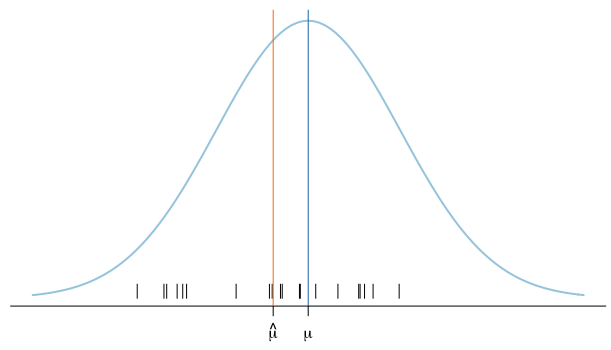
\includegraphics[width=0.8\hsize]{boot1}
	\caption{正規分布の平均値の推定.平均$\mu$の正規分布(水色線)からサンプルされたデータ点を軸上に黒線で図示している.標本平均を$\hat{\mu}$で示している.}
	\label{fig:boot1}
\end{figure}
モンテカルロ法で20点のデータを複数作り,それぞれで平均値を推定すると推定量$\hat{\mu}$の分布が得られる.
推定量の分布を\Figref{fig:boot2}に示す.
\begin{figure}[htbp]
	\centering
	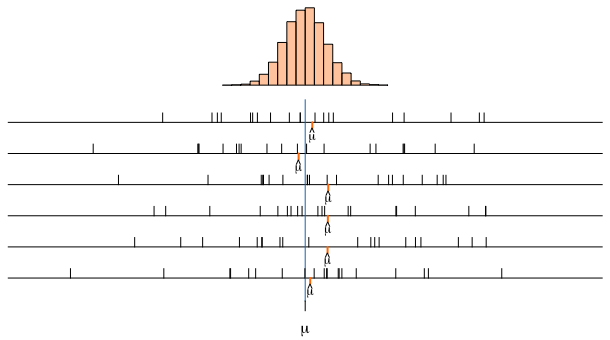
\includegraphics[width=0.8\hsize]{boot2}
	\caption{モンテカルロ法で20点のデータを複数作り,それぞれで平均の推定量$\hat{\mu}$を推定した図.上部のヒストグラムは$\hat{\mu}$の分布.}
	\label{fig:boot2}
\end{figure}
\Figref{fig:boot1}でサンプルされたデータ点から復元抽出を行い20点のデータを複数作成する.
このサンプルをブートストラップサンプルという.
ブートストラップサンプルそれぞれで平均値を推定すると推定量$\tilde{\mu}$の分布が得られる.
この時,真の平均は$\hat{\mu}$である.
推定量$\tilde{\mu}$の分布を\Figref{fig:boot3}に示す.
モンテカルロ法から作られたサンプルによる推定値の分布も示しているが,分布の平均$\mu$とデータ点の平均$\hat{\mu}$の差分ずれていることがわかる.
\begin{figure}[htbp]
	\centering
	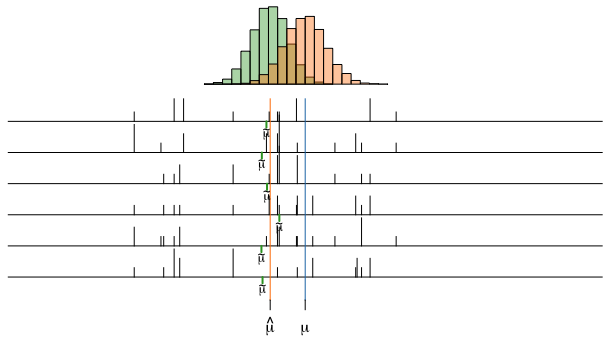
\includegraphics[width=0.8\hsize]{boot3}
	\caption{\Figref{fig:boot1}のサンプルからブートストラップサンプルを複数作成し,それぞれで平均の推定量$\tilde{\mu}$を推定した図.上部のヒストグラムは$\hat{\mu}$の分布(オレンジ)と$\tilde{\mu}$の分布(緑).}
	\label{fig:boot3}
\end{figure}
モンテカルロ法から作られたサンプルとブートストラップサンプルそれぞれの推定値の平均のヒストグラムを,それぞれの真の値を0としてずらしたものを\Figref{fig:boot4}に示す.
真の値での推定値のばらつきはほとんど同じである.
\begin{figure}[htbp]
	\centering
	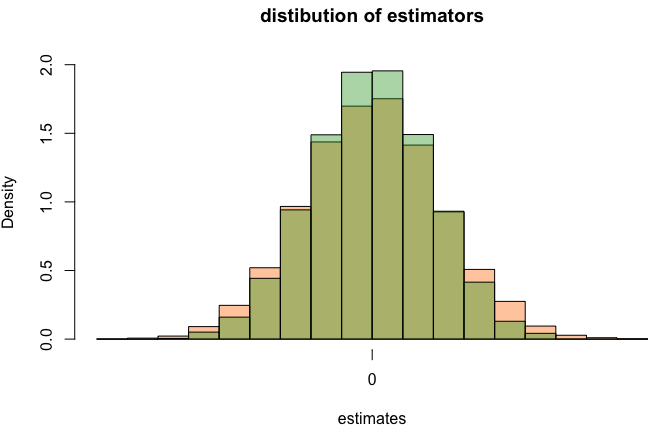
\includegraphics[width=0.8\hsize]{boot4}
	\caption{正規分布の平均値の推定.}
	\label{fig:boot4}
\end{figure}
これよりブートストラップ法では,データの分布によってどれだけ推定量がばらつくかを,観測データから得ることができる.
% データ$X$が分布$F$に従うとき,確率変数$R(X,F)$を推定する問題を考える.
% ブートストラップサンプル$X^*$を作成して,$R^* = R(X^*, \hat{F})$を推定すると,$R^*$の分布は$R$の分布を近似する.
% $F = \hat{F}$の時,$R^*$と$R$の分布は一致する.

\section{スペクトラルクラスタリング}
スペクトラルクラスタリングはクラスタリング手法の一つで,類似度行列からクラスタリングを行う.
類似度行列からグラフラプラシアンを求め,その固有ベクトルをk-meansなどでクラスタリングする.
スペクトラルクラスタリングはグラフカットとして解釈することができる.

具体的な手順を説明する.
類似度行列を$Q \in \mathbb{R}^{I \times I}$とする.
類似度行列$Q$から重み付き無向グラフの隣接行列を$R \in \mathbb{R}_+^{I \times I}$作成する.
隣接行列$R$は$Q$をそのまま用いる場合や,$k$近傍や$\varepsilon$近傍以外を0にすることで作成する.
またそのグラフの次数行列を$O \in \mathbb{R}_+^{I \times I}$とする.
次数行列$O$は対角行列でその対角成分は以下のように定義する:
\begin{equation}
	o_{ii} = \sum_{j=1}^I r_{ij}.
\end{equation}
グラフラプラシアンにはいくつか種類がある.
まず,正規化されていないグラフラプラシアンは以下のように定義されている:
\begin{equation}
	L = O - R.
\end{equation}
次に,正規化されたグラフラプラシアンには2種類ある:
\begin{align}
	L_{sym} &= O^{-\frac{1}{2}}LO^{-\frac{1}{2}} = I - O^{-\frac{1}{2}}RO^{-\frac{1}{2}}, \\
	L_{rw} &= O^{-1} L = I - O^{-1}R.
\end{align}
いずれかのグラフラプラシアンを使って\Alref{al:spectral}のアルゴリズムでクラスタリングを行う.
Luxburgは正規化されたグラフラプラシアンの方が良く,$L_{sym}$より$L_{rw}$の方が良いと述べている\cite{VonLuxburg}.

\begin{algorithm}
	\caption{スペクトラルクラスタリングのアルゴリズム}
	\label{al:spectral}
	\begin{algorithmic}[1]
		\Require{類似度行列$Q$,クラスタ数$k$}
		\Ensure{クラスタリング結果$B_1, \dots, B_k$}
		\State{隣接行列$R$を$Q$そのままを用いるか,$Q$の$k$近傍や$\varepsilon$近傍以外を0にして作成}
		\State{グラフラプラシアン$L$を計算する}
		\State{グラフラプラシアン$L$の固有ベクトルを求め,最初の$k$個$\mathbf{u}_1, \dots,\mathbf{u}_k$を取り出す}
		\State{行列$U \in \mathbb{R}^{I \times k}$を$\mathbf{u}_1,\dots,\mathbf{u}_k$を列に持つ行列とする}
		\State{行列$U$の行をk-meansでクラスタリングを行いクラスタを得る:$B_1, \dots, B_k$}
	\end{algorithmic}
\end{algorithm}

クラスタ数の決め方には様々な方法がある.
クラスタリング手法によらない方法には,安定性を見る方法\cite{Ben-Hur}やGap統計量\cite{Tibshirani}がある.
スペクトラルクラスタリングに特化した方法としては,固有値ギャップを見る方法\cite{VonLuxburg}がある.
固有値ギャップは固有値を小さい順にプロットした際に,急激に固有値が大きくなる箇所であり,その順位をクラスタ数とする.
